% !TeX spellcheck = en_GB
\documentclass{article}

\usepackage{float}
\usepackage[hidelinks]{hyperref}
\usepackage{graphicx}
\usepackage{caption}
\usepackage{tabu}
\usepackage{subcaption}
\usepackage{adjustbox}
\usepackage[utf8]{inputenc}
\usepackage[colorinlistoftodos,]{todonotes}
\usepackage{cite}
\usepackage[nottoc,numbib]{tocbibind}
\usepackage{pdfpages}
\usepackage{listingsutf8}



\newcommand{\newpar}{\bigskip\noindent}
\bibliographystyle{plain}
\presetkeys{todonotes}{inline}{}

\author{Anders Wind Steffensen (awis@itu.dk)\and Mikael Lindemann (mlin@itu.dk)\\\\Supervisor: Sebastian Risi (sebr@itu.dk)}
\title{Shortest Path in Undirected Unweighted Graphs using Evolvable Neural Turing Machine}

\begin{document}
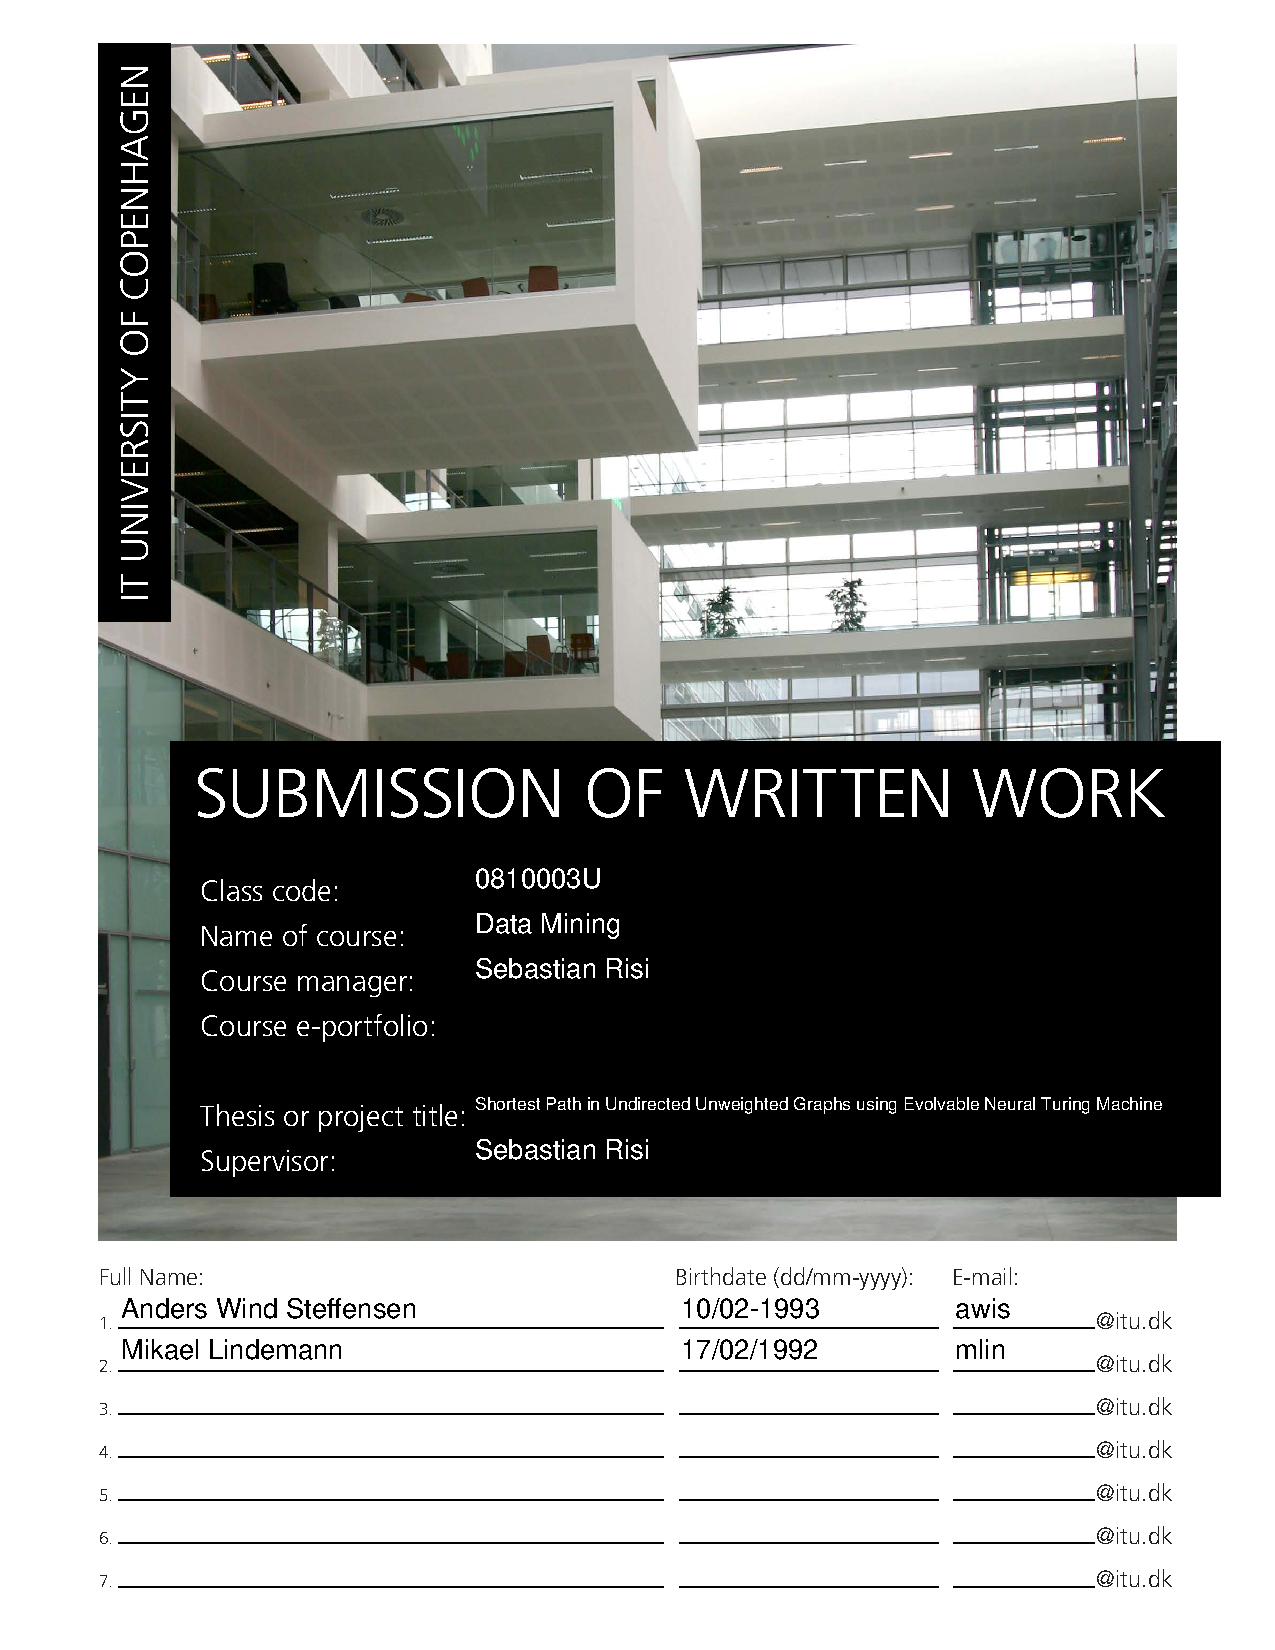
\includepdf{frontpage}
\maketitle
\tableofcontents
\listoftodos
\newpage
% !TeX root = report.tex
% !TeX spellcheck = en_GB

\section{Introduction}
Finding the shortest path in a graph is one of the most well studied algorithmic graph problems. Solutions for the problem origin back to the late 1950's. Finding the shortest path has a long list of applications from transport and routing tables in networks to being an essential subroutine of many more advanced graph algorithms. 
In recent years neural networks has gained more and more traction in the artificial intelligence and machine learning fields. This increased focus on neural networks is both due to theoretical breakthroughs but also the more widespread adoption and advancement of graphical processing units. Neural networks are most often used for classification, finding heuristics and as the decision mechanism for artificial agents.

\newpar One of the most criticized problems of neural networks and machine learning in general is that agents are inherently single purpose and problems different from what is trained on is often not handled very well.

\newpar With the introduction of neural networks with memory more domains should be feasibly solvable. In \cite{graves2016hybrid} a differentiable neural computer was shown to be able to find the shortest path in the London underground by using memory to store variables and information about the graph. In \cite{greve2016evolving} an evolutionary version of the neural Turing machine was introduced. Evolutionary neural networks does not require every part of the problem to be differentiable and allows reward based learning.

\newpar In this report we want to examine how well these evolutionary neural Turing machines can handle the shortest path problem on undirected, unweighted graphs. Both acyclic and recurrent neural networks will be examined.

\newpar The source code of the experimentation can be found at\\ \href{https://github.com/Awia00/Data-Mining/tree/master/Group%20Project/NeatBFS/src/NeatBFS}{www.github.com/Awia00/Data-Mining}.
% !TeX root = report.tex
% !TeX spellcheck = en_GB

\section{Background}
\subsection{Graphs}
A \textit{graph} $G(V,E)$ is data-structure which consists of a set of \textit{vertices} $V$ and a set of \textit{edges} $E$ where an edge is a pair of vertices $(u,v)$. An \textit{undirected graph} implies that if edge $ (u,v) $ exists then $ (v,u) $ exists in the graph. An \textit{unweighted graph} every edge is equal in the cost to traverse it.
Two vertices are \textit{adjacent} if they are part of the same edge $ e $. A \textit{path} $ P $ is a ordered set of edges such that every consecutive edge shares a vertex. To vertices $ u $, $ v $ are \textit{connected} if there exist a path between $ u $, $ v $.

\newpar In an undirected unweighted graph the length of a path P is $|P|$. A shortest path between two vertices  $u$, $v$ is a path $P$ connecting  $u$, $v$ of the smallest length. The Breadth First Search (BFS) algorithm can find the shortest path in time $\mathcal{O}(n+m)$ where $n=|V|$ and $m=|E|$. To be able to solve this combinatorial problem for which the exhaustive search space is $n!$ the BFS algorithm uses a queue to store previously visited vertices and a map of the vertices and which vertex would come before it in the shortest path.

\subsection{Neural Networks}
A \textit{neural network} is an approximation method for \textit{n} dimensional functions. Neural networks consists of a collection of \textit{layers} $L_1 .. L_n$ where $L_1$ is the \textit{input layer}, $L_2 .. L_{n-1}$ are \textit{hidden layers}, and $L_n$ is the \textit{output layer}. Each layer $L_i$ consist of a number of \textit{neurons}. A neuron is connected to other neurons in the layer before and after its own layer. Neurons can send signals to other neurons it is connected to. The strength of a signal is specified by a \textit{signal function} of a neuron. Neurons gets \textit{activated} and sends a signal if itself has become activated a \textit{threshold} amount by other neurons. The signal function is based on a \textit{formula}, a \textit{weight} and a \textit{bias}. 

\newpar The \textit{feed forward algorithm} activates the neurons of the input layer based on some input data, whom in return activates the neurons of the next layer and so on. The values of the output layer is then read. The \textit{back-propagation algorithm} calculates the error of the output neurons compared to the input data and corrects it based on a function. The errors are then back-propagated through the layers. By running the feed forward and back-propagation algorithms in combination with enough data, almost any function can be approximated.

\newpar It is also possible for a neural network to be recurrent. These kinds of networks allow a neuron to be connected to itself, other neurons in the same layer, or maybe the neurons of the entire network, depending on the configuration.

\newpar A \textit{one hot encoding} of a nominal data point, is a conversion of the data point into a bit array $A$ with the length $n$, where $n$ is the number of possible nominal values. Each of the nominal values are then assigned a label $i \in \{0 .. n-1\}$. For a nominal value with label $i$ only $ A[i] $ is $1$. All other elements in $A$ is $0$. This encoding is often used for neural networks, as each element of $A$ can be used as the input for a single neuron in the input layer of a neural network.

\subsection{Evolutionary Neural Networks}
Evolutionary neural networks is a method of training the weights of a neural network based on evolutionary algorithms. These networks can be trained without using supervised learning but reward based learning where a fitness function describes how well the network does in the specific instance. The use of evolutionary algorithms means that high performing neural networks are the base for the next generations, rather than choosing arbitrary or completely random networks in each generation.

\subsubsection{NeuroEvolution of Augmenting Topologies (NEAT)}
Whereas most other Evolutionary Neural Network algorithms, start from a randomly seeded network with a fixed topology, NEAT evolves the topology from the minimal network, where no hidden neurons exist.

\newpar NEAT has a few main components, that is used to improve over previous neuroevolution algorithms:

\begin{itemize}
	\item Innovation numbering
	\item Speciation
	\item Incremental growth from minimal structure
\end{itemize}

\newpar NEAT uses a technique called innovation numbering, in order to distinguish or compare genes between genomes. The technique is used both when mating, that is, pairing two phenotypes in order to produce new outspring, and when grouping the phenotypes into species.

\newpar The notion of species is used to protect innovative but untrained structures in new genomes. The idea is that, when a new structure has been introduced, it might not have good weights associated, which means that it will initially perform worse than older and trained genomes without this structure. Instead of having all genomes compete against each other, the genomes are divided into species, where the genomes inside a specie compete against each other. This allows the innovative mutations to last some generations, so they can prove, or disprove, their worth.

\newpar Further details about the NEAT algorithm can be found in \cite{stanley2002evolving}.

\subsection{Evolvable Neural Turing Machine (ENTM)}
In \cite{greve2016evolving} Greve et. al. introduces the Evolvable Neural Turing Machine as an extension of the Neural Turing Machine (NTM, \cite{graves2014neural}), with the difference that the ENTM does not require the network to read through the entire memory bank at each time-step, as the NTM does. Furthermore the memory bank can be theoretically unlimited in the ENTM setup.

\newpar With this change comes also a different way of addressing the memory bank. The Turing Machine part of ENTM has four operations that can be performed on the memory banks read/write-head:

\begin{enumerate}
	\item Write - Writes the content of the write vector to the current position in the memory bank.\footnote{This is a simplification. The content is interpolated with the existing vector.}
	\item Content Jump - Moves the read/write head to the memory bank position that is most similar to the write vector.
	\item Shift - The read/write head can be shifted one position to the left or right, or it can be kept at the current position.
	\item Read - The content of the current position is used as input for the next artificial neural network in the next time-step.
\end{enumerate}

\newpar Furthermore the ENTM is trained and evolved using NEAT, whereas the NTM uses gradient descent. This enforces looser requirements to the structure and activation functions of the neural network.

\newpar Greve et. al. shows that the ENTM is able to solve simple algorithm tasks such as the copy task, and the continuous T-maze task.

% !TeX root = report.tex
% !TeX spellcheck = en_GB

\section{Experiment}
The problem definition is as follows: 
Given a graph $G$, a source vertex $s$, and a goal vertex $t$, find the shortest path from $s$ to $t$ in $G$.

\newpar We have restricted the problem to instances where a path between $s$ and $t$ exists.

\subsection{Instances}
In order to feed the instance into the network, we use an encoding of the adjacency matrix of the graph, where each edge has the value 1, and each non-edge has the value 0. The source and goal vertices are one-hot encoded. See \autoref{fig:input:encoding} for an example. The output of the ENTM is interpreted as a one-hot encoding of the next vertex on the path to the goal. After each step the source vertex is updated to the previously outputted vertex in the new input to the ENTM.

\begin{figure}[ht]
	\centering
	\begin{subfigure}{.5\textwidth}
		\centering
		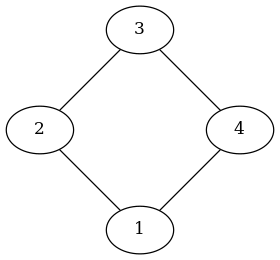
\includegraphics[width=\textwidth]{figures/encoding.png}
		\subcaption{}
	\end{subfigure}%
	\begin{subfigure}{.5\textwidth}
		\centering
		\begin{tabular}{|c|c|c|c|c|}
			\hline
			&\textbf{1}&\textbf{2}&\textbf{3}&\textbf{4}\\\hline
			\textbf{1}&0&1&0&0\\\hline
			\textbf{2}&1&0&1&1\\\hline
			\textbf{3}&0&1&0&1\\\hline
			\textbf{4}&0&1&1&0\\\hline
		\end{tabular}
		\subcaption{}
	\end{subfigure}\par\bigskip
	\begin{adjustbox}{center}
		\begin{subfigure}{1.3\textwidth}
			\centering
			\begin{tabu}{|c|c|c|c||c|c|c|c||c|c|c|c||c|c|c|c|[2pt]c|c|c|c|[2pt]c|c|c|c|}
				\hline
				0&1&0&0&1&0&1&1&0&1&0&1&0&1&1&0&1&0&0&0&0&0&0&1\\\hline
			\end{tabu}
			\subcaption{}
		\end{subfigure}
	\end{adjustbox}
	\caption{(a) Shows a simple graph, (b) its adjacency matrix and (c) an encoding of the entire instance where $s=1$ and $t=4$. The array contains the flattened adjacency table, the one-hot encoding of $s$, and the one-hot encoding of $t$}
	\label{fig:input:encoding}
\end{figure}

\newpar The instances are generated in a manner which tries to avoid over fitting and support general solutions. This is done by using randomly generated graphs with certain restrictions. The graph must contain a path of a given length to ensure a certain level of complexity. This level of complexity filters out optimal strategies on non general case graphs such as graphs with paths of length 1 where the optimal solution is outputting the goal vertex. Generating these graphs is done by picking two random vertices $ s $ and $ t $ and randomly pick vertices that forms a path from $ s $ to $ t $. The remaining vertices are then connected to the set of explored vertices randomly. This ensures that the ENTM cannot just follow edges but need to explore branches of the graph. The generated graphs are of fixed size to ensure neural network compatibility.

\subsection{Fitness}
The fitness function is defined as a summation of scores for the output of each step on the shortest path. The function $ DistTo(u) $ is defined to return the shortest distance from vertex $ u $ to the goal vertex. The vertex $ current $ describes the vertex which was given to the network and $ next $ denotes the network's choice of the next vertex along the path to the goal. The following scores are given in each step:

\begin{itemize}
	\item[] 1 point: if $ DistTo(next) > DistTo(current) $
	\item[] 2 points: if $ DistTo(next) = DistTo(current) $
	\item[] 4 points: if $ DistTo(next) < DistTo(current) $
\end{itemize}

\noindent In the case that one step resulted in a move where no edge exists the overall score is set to 0, and no further steps are performed. 

Note that the instance generation defined above does not create any cycles and therefore the score 2 will never be given.

\newpar The motivation for these scores is to reward neural networks that understand the underlying graph problem more than a network that chooses arbitrarily.

\newpar The final score is normalized by the following formula $ \frac{score}{DistTo(source)*4} $ where the denominator is the  maximum score. Note that $ DistTo(source) $ is the maximum number of moves allowed.

\subsection{The Experiments}
To assess and measure how well the shortest path problem is solved, four different types of experiments are performed. The first experiment uses the NEAT framework to train and build neural networks with recurrent connections. The next experiment uses the ENTM extension of the NEAT framework using recurrent neural networks. The memory is unlimited (within the bounds of the host machine), the write vector size is 10 and the default jump mechanism introduced in \cite{luders2017continual} is used. The two experiments are repeated on acyclic topologies.

\newpar All experiments uses the exact same configuration for NEAT and runs on the same instances to make them comparable. Each configuration uses a population of 500 divided into 30 species. Each phenotype is tested on 25 unique graphs per generation. All graphs have 10 vertices and 9 edges, of which 5 are on the path between the source and the goal. An example configuration can be seen in \autoref{appendix:sharpneat:configurations}. The appendix also contains the changes between the different experiments.
% !TeX root = report.tex
% !TeX spellcheck = en_GB

\section{Results}
The results of the experiments can be seen on Figures \ref{experiments:graph:1}, \ref{experiments:graph:2}, \ref{experiments:graph:3} and \ref{experiments:graph:4}.\footnote{The data points behind the graphs can be found in the file \textit{All Runs.xslx}.} The $x$ axis shows the generation, and the $y$ axis shows the champion fitness achieved for that generation in the run.

\begin{figure}[H]
	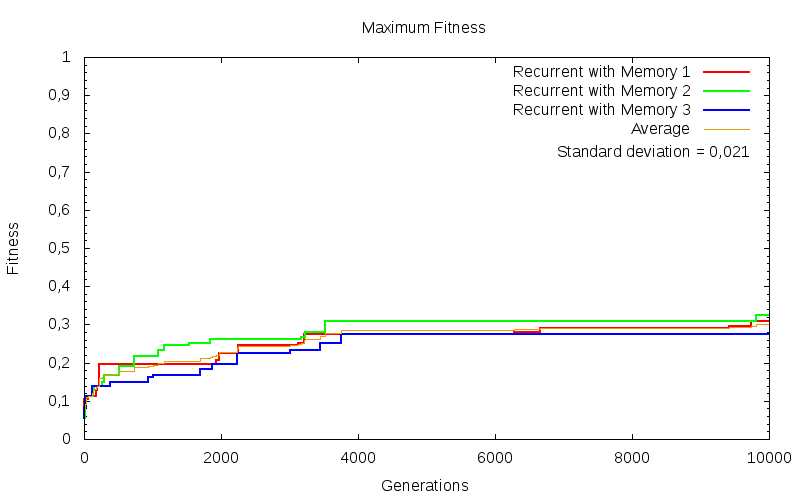
\includegraphics[width=\textwidth]{figures/recurrentmemory.png}
\caption{Graph of the results when using recurrent networks with enabled memory bank}
	\label{experiments:graph:1}
\end{figure}
\begin{figure}[H]
	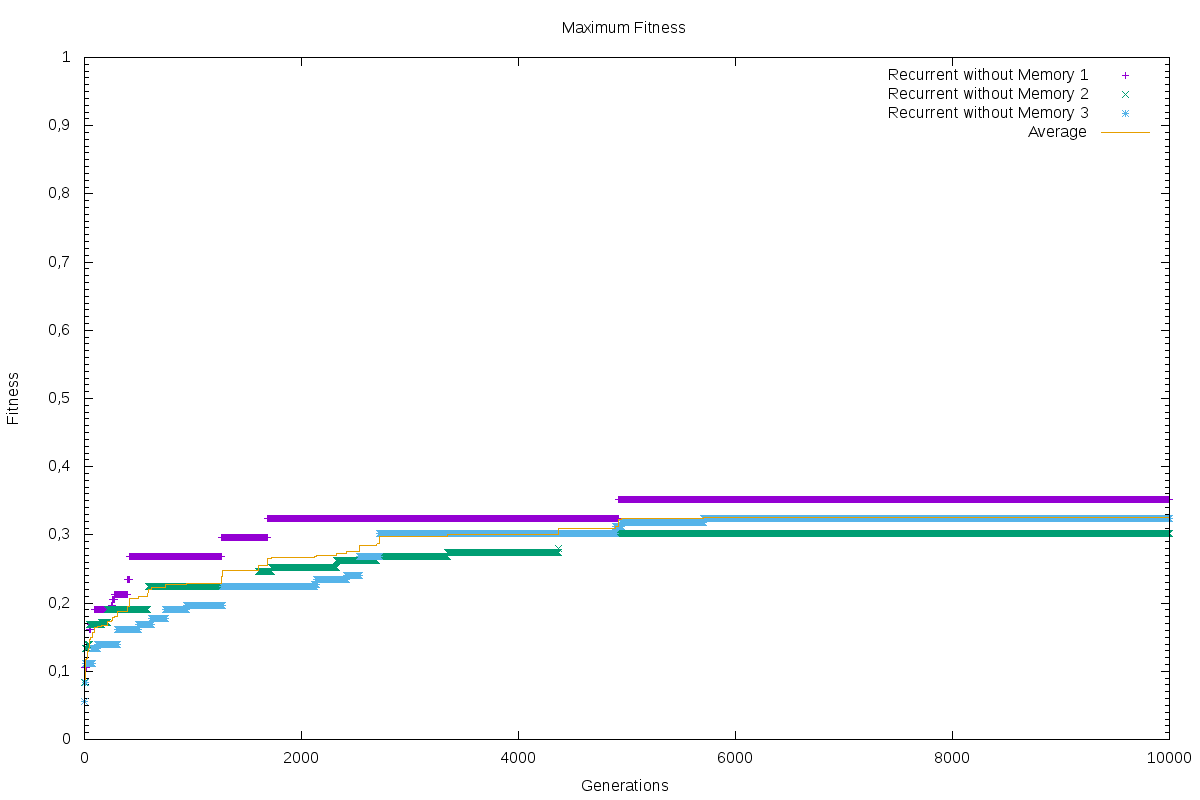
\includegraphics[width=\textwidth]{figures/recurrentnomemory.png}
	\caption{Graph of the results when using recurrent networks with disabled memory bank.}
		\label{experiments:graph:2}
\end{figure}

\begin{figure}[H]
	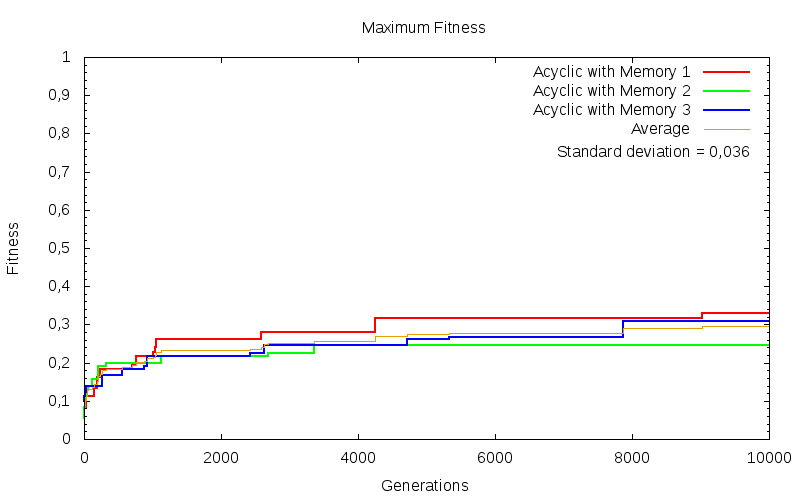
\includegraphics[width=\textwidth]{figures/acyclicmemory.png}
	\caption{Graph of the results when using acyclic networks with enabled memory bank.}
	\label{experiments:graph:3}
\end{figure}
\begin{figure}[H]
	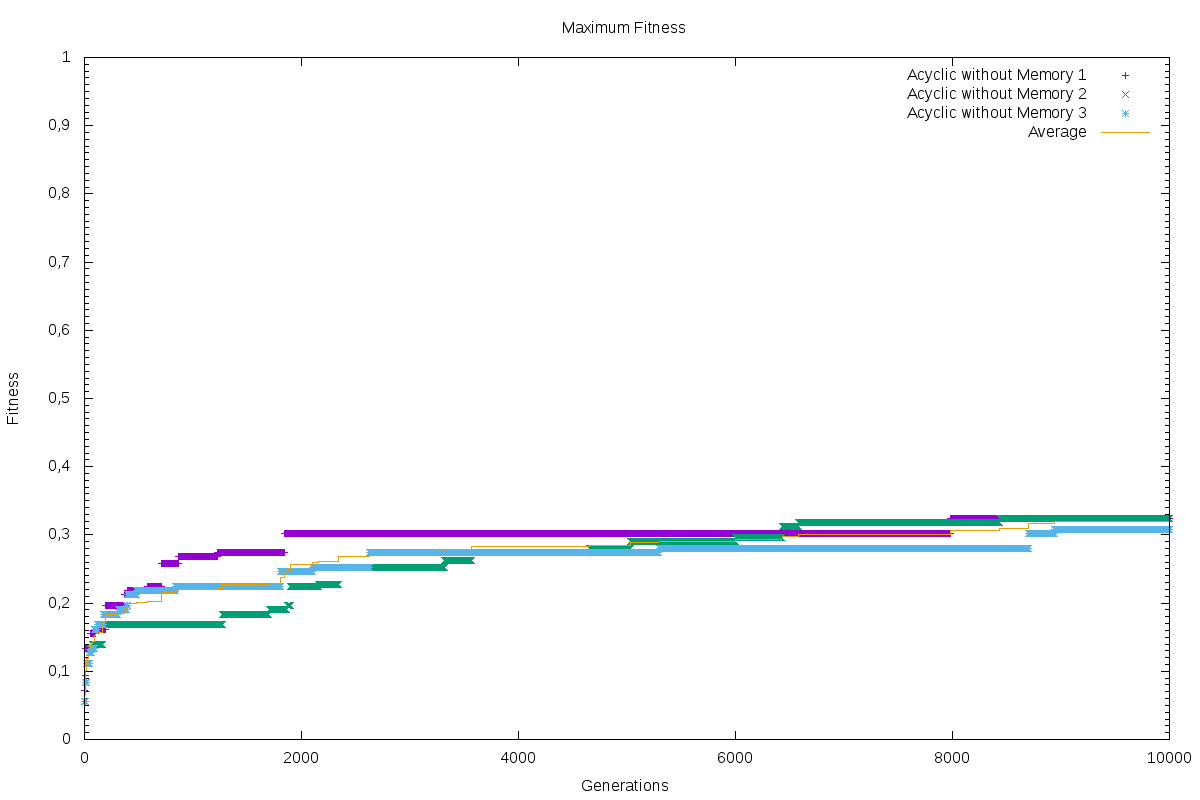
\includegraphics[width=\textwidth]{figures/acyclicnomemory.png}
	\caption{Graph of the results when using acyclic networks with disabled memory bank.}
	\label{experiments:graph:4}
\end{figure}

\begin{figure}[ht]
	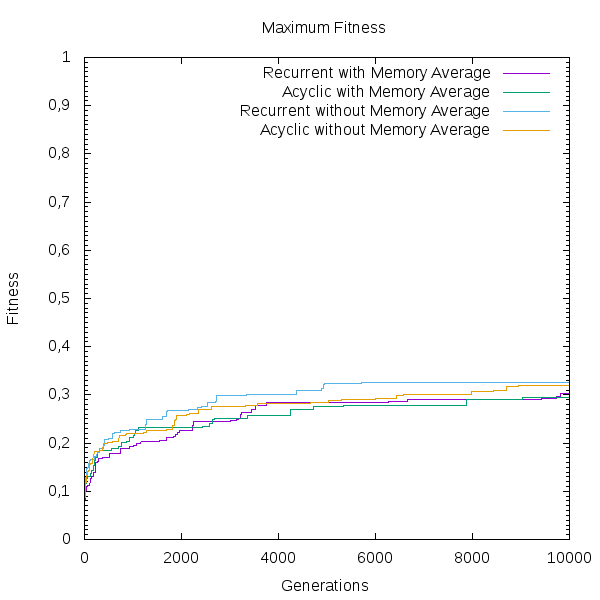
\includegraphics[width=\textwidth]{figures/averages.png}
	\caption{Averages over three runs of all configurations. Note that the y-axis has been truncated to make it easier to distinguish the different runs.}
	\label{experiments:graph:average}
\end{figure}

\newpar To compare the different experiments their averages are shown in \autoref{experiments:graph:average}. At generation 10.000 the averages show that both kinds of topologies find a better performing neural network when the Turing-functionality is turned off by a small margin of around 2\%.

\clearpage
% !TeX root = report.tex
% !TeX spellcheck = en_GB

\section{Analysis}
From the results above it seems that the structure of our input does not allow for good results.

\newpar Recurrent and acyclic neural networks as well as Turing enabled and disabled networks never (in 10.000 generations) achieve higher fitness than approximately 0.35. To put the value into perspective the result is compared to three suboptimal strategies.\footnote{We have included an Excel sheet to the submission of the report, where the calculations can be seen. The file is named Strategies.xlsx.} A strategy where moves are picked randomly including non-edges will result in an average fitness of 0.000126. A strategy which randomly picks legal moves will get an average fitness of 0.67 and a strategy which always moves away from the goal will get a fitness of 0.25. The span between these numbers are great, and it is clear that as soon as a strategy learns to not pick non-edges the fitness greatly increases. The observation is therefore that the champion must have some understanding of the graph but only enough so that it most of the time does not pick non-edges. The strategy of always moving away from the goal is in some sense just as hard a problem as the shortest path to the goal, therefore it is not likely that the champion uses this strategy. 

\newpar To further analyse the champions we examine the behaviour of the champion on a collection of graphs. The champions seem to pick a lot of non edges but in a lot of instances the weights of the output contains high values for multiple decisions. In \autoref{table:analysis:1} an action of one of the champions with memory can be seen. It decides to move to vertex 3 which is faulty and results in score 0 on the entire iteration. But it is interesting to see that the only valid move of the instance also has a high score which only differs in the 5th decimal. This supports the indication that the network in general has higher chances of picking correct moves than a totally uniform random strategy.

\begin{table}
	\centering
	\begin{tabular}{|l|l|l|}
		\hline
		Move:&	decision & score for decision\\
		\hline
		0:&	0.5 & 0 \\
		\hline
		1:&	0.5	& 0\\
		\hline
		2:&	0.5	& 0\\
		\hline
		3:&	0.99999 & 0\\
		\hline
		4:&	0.5	& 0\\
		\hline
		5:&	0.5	& 0\\
		\hline
		6:&	0.99392 & 0\\
		\hline
		7:&	0.99994 & 4\\
		\hline
		8:&	0.5 & 0	\\
		\hline
		9:&	0.5 & 0\\
		\hline
	\end{tabular}
	\caption{The output array of a network. The network is on vertex 1 goal is 0. Should move to 7 as it is the only possible edge. Chooses to move to 3 which is connected to 0.}
	\label{table:analysis:1}
\end{table}

\newpar One possible reason for this, might be that the encoding of the problem is not feasible for the ENTM. If we compare our encoding to that of the Copy Task from \cite{greve2016evolving}, they made sure to signal the network when starting a new assignment and when asking it to return the content back. Also, they supplied the input in multiple time-steps rather than giving the entire sequence all at once.

\newpar The shortest path problem differ from the Copy task in that the memory bank should not only be used to store content as provided. It should be used to model some structure that would allow for the planning problem to be performed. Since we ask for output in every iteration (also the first), we don't allow the ENTM to preprocess anything. This might be another place to tweak the problem encoding. Further experiments might try to feed the graph in multiple steps and different encodings, and train the network to signal when it is ready to answer on the shortest path problem.
% !TeX root = report.tex
% !TeX spellcheck = en_GB

\section{Conclusion}
We were unsuccessful in training an evolutionary neural Turing machine to be able to find the shortest path in a undirected unweighted graph. On graphs with 10 vertices and 9 edges, where the shortest path between the source and target has a length of 5, only a fitness value of $\approx0.35 $ was achieved. This result outperforms a strategy of randomly picking moves by a large factor but is only half as good as randomly picking legal moves. The network was not able to fully learn how to recognize edges in the graph but indicated higher values for the correct move than the average case. 
The difference between the neural Turing machines and the regular neural networks was insignificant and in average the networks without memory achieved a higher fitness. 

\newpar There is a lot of possible extensions and areas left unexplored which could provide more interesting results. Allowing the network to read and write memory multiple times in one activation or changing the structure of experiments might allow the networks to better plan ahead. Also, the ENTM might need a few intermediate activations in order to update the memory bank, before it is possible for it to give the correct result in subsequent time-steps.

\newpage
\bibliography{bibliography}

\newpage

\appendix
\section{SharpNEAT Configuration Files}
\label{appendix:sharpneat:configurations}
\todo{Configuration files}
\subsection{Configuration with memory}
\lstinputlisting[numbers=left,breaklines=true,basicstyle=\footnotesize,stepnumber=1,frame=single]{../NeatBFS/src/NeatBFS/Config/SingleStepShortestPathTask/PathWithRandom/10vertices5edgesWithMemory.xml}

\subsection{Configuration without memory}
\lstinputlisting[numbers=left,breaklines=true,basicstyle=\footnotesize,stepnumber=1,frame=single]{../NeatBFS/src/NeatBFS/Config/SingleStepShortestPathTask/PathWithRandom/10vertices5edgesWithoutMemory.xml}
\end{document}
